\label{driver-notification}
\subsubsection{Purpose}

After a taxi driver has informed the system about his/her availability (section~\ref{taxi-availability})
he/she will be able to receive ride request notifications. The taxi driver receives the notifications on his/her cell phone and has one minute to accept or reject the request. If after one minute the request is not answered, the system will consider the request as refused.

\subsubsection{Scenario 1}
Travis, who suffers from chronic insomnia, every night waits in his taxi for an incoming request. When a user requests a taxi, the system processes the request and decides which taxi driver to send.

For a new incoming request, the system chooses Travis, who is on the top of the queue and in the same taxi zone of the passenger. The system sends him a notification on his mobile app. Travis reads the message which reports location and time of the meeting and decides to accept the request pushing the appropriate button on the display.

The system acknowledges the decision and waits for Travis to notify that the passenger is on board (last part of~\ref{standard-call}).

\subsubsection{Scenario 2}
The system receives a new incoming request from a user and selects Frank Martin as designated taxi driver (section~\ref{taxi-availability}).
The system sends him a notification and waits for the reply.

Frank has just finished a very demanding ride, so he decides to refuse the request using the interface of the app. The system receives Frank's decision and looks for another available taxi on the same taxi area.

\begin{figure}
\begin{center}
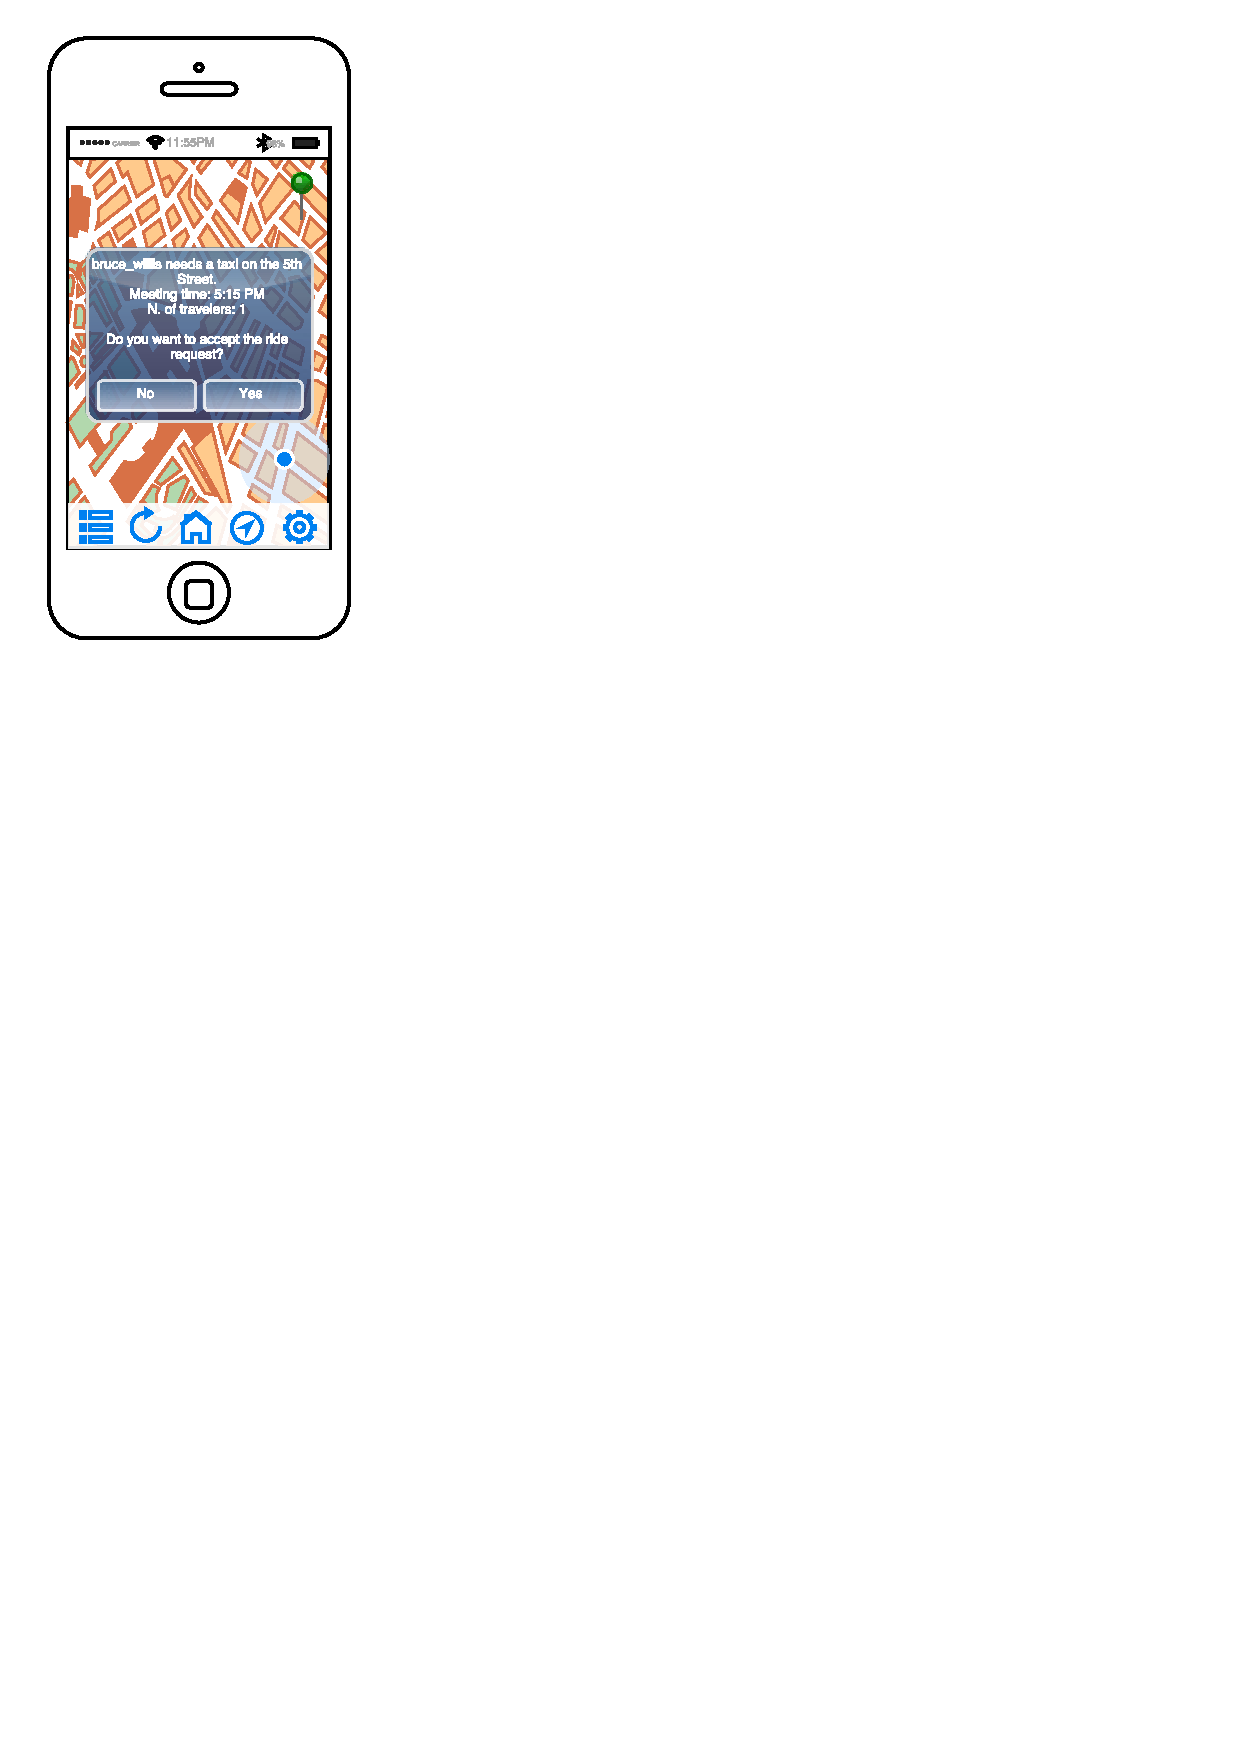
\includegraphics[width=0.5\textwidth]{mockup/RideRequest.pdf}
\caption{Concept of the ride request notification.}
\label{fig:mockup-riderequest}
\end{center}
\end{figure}

\subsubsection{Use case}
The use case for a driver notification is shown in~\autoref{usecase-drivernotification}.

\begin{table}
\begin{center}
\begin{tabular}{| l | p{0.6\textwidth} |}
\hline
Actor & Taxi driver \\
\hline
Goal & Goal~\ref{g-notify}
\\
\hline
Input condition & The system informs the taxi driver about a new request.  \\
\hline
Event Flow & \begin{enumerate}
	\item The system informs the taxi driver about a new request, specifying time and location of the ride.
	\item The taxi driver sees the information on his cell phone and chooses whether to accept or to refuse the request.
	\item If the request is accepted, the system dequeues the taxi and marks it as busy, otherwise it sends the request to the next taxi.
	\item When someone has accepted, the system notifies it to the passenger specifying the arrival time of the taxi.
	\end{enumerate}
\\
\hline
Output condition & The system informs the passenger about the estimated time of arrival of the taxi. \\
\hline
Exception &
\begin{enumerate}
	\item No taxi replies to the request: an error message is displayed to the user.
	\item If after a minute the taxi driver has not sent any response, the system considers the request refused and moves on to the next taxi driver in queue.
\end{enumerate}
\\
\hline
\end{tabular}
\end{center}
\caption{Use case for driver notification.}
\label{usecase-drivernotification}
\end{table}

\subsubsection{Response sequence}
The use case associated to the response sequence is shown in~\autoref{fig:sequence-taxicall-refused}.

\subsubsection{Associated functional requirements}
\begin{enumerate}
\item The app must show any incoming request notification to first taxi driver in the queue of the same zone of the passenger.
\item The system allows the taxi driver to accept or decline the request using the app.
\item The app must produce sounds or visual notifications as the taxi driver has chosen.
\item The system has to provide the taxi driver with information about the time and place of the meeting with the passenger.
\item The system gives to the taxi driver one minute to reply. Else, the request is automatically refused.
\item The request notification shall contain the following information:
\begin{enumerate}
	\item number of travelers;
	\item location of the passenger;
	\item username of the passenger;
	\item estimated time of the meeting with the passenger.
\end{enumerate}
\end{enumerate}
